\documentclass[]{article}

% Import packages
\usepackage[fleqn]{amsmath}
% \usepackage{mathtools}
\usepackage{graphicx}
\usepackage[export]{adjustbox}
% \usepackage{tikz}
\usepackage{xcolor}

% \usetikzlibrary{positioning,shapes,arrows}

% Page initialization
\setlength{\topmargin}{-.3 in}
\setlength{\oddsidemargin}{0in}
\setlength{\evensidemargin}{0in}
\setlength{\textheight}{9.in}
\setlength{\textwidth}{6.5in}
\pagestyle{empty}

%==============================================================%
%------------------------START-DOCUMENT------------------------%
%==============================================================%
\begin{document}

%----------------------------HEADER----------------------------%

\begin{center}
    {\Large AERO 422 Homework \#3}\\ % Homework number
    \vspace{0.2 cm}
    Instructor: Vedang Deshpande\\ % Instructor name
    \vspace{0.2 cm}
    Due: October 05, 2021 at 12:00a.m.\\ % Due date
    \vspace{0.2 cm}
    Fall 2021\\ % semester
    \vspace{0.2 cm}
    (\textbf{28 Points})\\
\end{center}

\vspace{0.2 cm}

\begin{enumerate}

    %---------------------------PROBLEM-1--------------------------%
    \item A block diagram for a spacecraft docking control problem is given by
    % insert image
    \begin{figure}[h]
        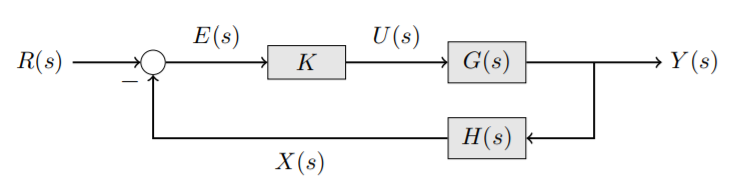
\includegraphics[scale=0.8,center]{AERO_422_HW3_P1.png}
        % \caption{Convolution integral (reference for problem 4)}
    \end{figure}
    \\where $K$ represents the controller. It is important to keep in mind that this is a docking problem, so overshooting (going past) the reference input is not desired.

    \begin{enumerate}
        \item (\textbf{1 point}) Evaluate the transfer function from $U(s)$ to $Y(s)$ if the input/output relationship satisfies
        $$m\ddot{y}(t) + c\dot{y}(t) = u(t)$$
        \textcolor{blue}{
        Solution in other document.
        }

        \item (\textbf{1 point}) Evaluate the transfer function from $Y(s)$ to $X(s)$ if
        $$\dot{x}(t) + \tau x(t) = \tau y(t)$$
        \textcolor{blue}{
        Solution in other document.
        }

        \item (\textbf{2 points}) Consider the closed loop transfer function $T(s)$, such that $Y(s) = T(s) \cdot R(s)$. $T(s)$ has the form, 
        $$T(s) = \frac{a_1s + 60}{b_3s^3 + b_2s^2 + b_1s + 60}$$        
        Determine the values of $a_1$, $b_3$, $b_2$, $b_1$ is the text boxes below when
        $K = 5$, $m = 2$, $c = 7$, and $\tau = 12$.\\\\
        \textcolor{blue}{
        Solution in other document.
        }

        \item (\textbf{12 points}) Consider three cases of parameter values:\\\\
        Case 1: $K = 30$, $m = 2$, $c = 7$, $\tau = 0.2$\\
        Case 2: $K = 5$, $m = 2$, $c = 7$, $\tau = 12$\\
        Case 3: $K = 10$, $m = 2$, $c = 7$, $\tau = 0.1$\\\\
        For all cases,\\\\
        i.) Plot $y(t)$ if $r(t) = 1(t), t \geq 0$. You may use the "step" command in MATLAB.\\\\
        ii.) Plot the pole-zero map of $T(s)$ using MATLAB.\\\\
        iii.) For each case, determine whether or not the system is stable.\\\\
        iv.) For each case, determine whether or not this parameter set is acceptable for the problem application we have considered.
        \textcolor{blue}{
        }
        
    \end{enumerate}

\end{enumerate}

\end{document}